Low-rank adaptation (LoRA)~\citep{hu2022lora} makes it cheap to train many
specialised versions of one base model, so it is attractive to merge several
of them back into a single set of weights. Many merging methods exist: task
arithmetic~\citep{ilharco2023task}, sign election (TIES)~\citep{yadav2023ties},
random sparsification (DARE)~\citep{yu2024dare}, subspace alignment
(KnOTS)~\citep{stoica2025knots}, whitening (TSV-M)~\citep{gargiulo2025tsv},
least-squares solvers in the RegMean line~\citep{jin2023regmean,tam2024mats},
and data-free methods such as WUDI-Merging~\citep{cheng2025wudi}, which solves
a least-squares problem built from the task updates themselves. These methods
are compared mostly by benchmark averages, and the comparisons are unstable. A
method that works on one set of adapters can fail on another, and there is no
way to tell in advance which will happen.

This paper studies one property of a set of adapters that is fixed before
training starts and is almost never reported. LoRA writes each update as $BA$.
It starts $B$ at zero and draws $A$ at random. A \emph{cohort} is the set of
$T$ adapters to be merged, and the random seed in force when the adapters are
created decides whether they share \emph{one} $A$ or draw $T$ independent
ones. Because $B = 0$ at the start, $A$ moves little during training: about
$13\%$ of its norm in our measurements. Adapters that start from the same $A$
therefore stay close to it. A single global seed is the natural choice when
the seed is meant to make runs reproducible, and it gives every adapter of a
cohort nearly the same input subspace, whatever its task
(Figure~\ref{fig:concept}).

\begin{figure}[pos=tbp]
\centering
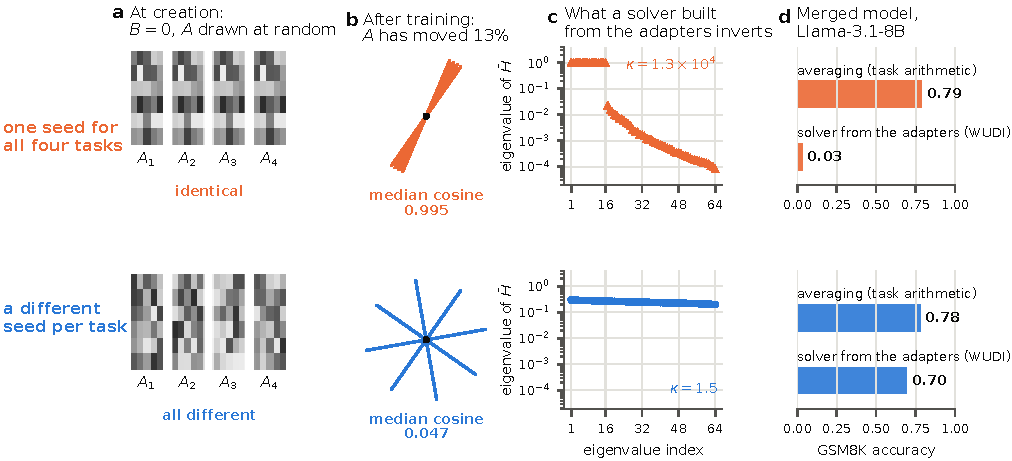
\includegraphics[width=\textwidth]{nc/figures/fig0_concept.pdf}
\caption{What a shared initialisation does, on Llama-3.1-8B. Top row: the
four adapters of a cohort are created from one random seed. Bottom row: each
task has its own seed. \textbf{(a)} LoRA starts $B$ at zero and draws $A$ at
random, so one seed gives four identical $A$ (an illustration with small
random matrices). \textbf{(b)} Training moves $A$ by only $13\%$ of its norm,
so adapters that start together stay together. The median principal cosine
between their input subspaces is $0.995$, against $0.047$ with a seed per
task (a two-dimensional sketch of rank-$16$ subspaces; the cosines are
measured). \textbf{(c)} The $64$ eigenvalues of $\bar H$, the matrix that a
least-squares merge built from the adapters has to invert, in one layer. With
one seed, $16$ sit near $1$ and the other $48$ fall to between $10^{-2}$ and
$10^{-4}$, so the condition number $\kappa$ is about $10^{4}$.
\textbf{(d)} GSM8K accuracy of the merged model, the mean over three cohorts
per row. Averaging the adapters works in both rows. WUDI-Merging, a published
merge that solves a least-squares problem built from the adapters, fails when
they share a seed.}
\label{fig:concept}
\end{figure}

Our lead result concerns a published method. WUDI-Merging needs no data, and
its authors minimise its objective with an optimiser that stops early instead
of solving the system. We expected the early stopping to act as an implicit
regulariser, and we registered it as protective. It is not. Run exactly as its
authors run it, WUDI leaves a worst-task loss excess (the merged model's extra
loss on its worst task) $4.7$ to $47.6$ times larger on cohorts with a shared
$A$ than on cohorts with independent ones. This holds on all four base models
we tested. On GSM8K the shared cohorts score $0.034$ against $0.695$ on
Llama-3.1-8B, and on HumanEval they score zero on two of the four bases. We had
written in advance that this outcome, if it occurred, would become the lead
result. It belongs to a class that we can state precisely. On language models,
a shared $A$ breaks every merge we tested that solves a least-squares problem
whose matrix is built from the adapters alone, in closed form or by gradient
descent. It breaks no other merge we tested.

We make four contributions.

\begin{enumerate}[leftmargin=*,itemsep=2pt,topsep=3pt]
\item \textbf{The collapse, measured.} On four base models with 7 to 9 billion
parameters, sharing the initial $A$ moves the median principal cosine between
task subspaces from about $0.05$ to above $0.99$. A registered ablation shows
that the seed in force when the adapters are created decides the regime by
itself; the dropout masks do not. The collapse holds at every task count and
rank we tested, and under each of seven changes to training. It also arises
without a shared seed: from PiSSA initialisation~\citep{meng2024pissa}, and
from training every task on from one existing adapter. It holds for DoRA and
for adapters on CLIP ViT-B/32 (\S\ref{sec:collapse}).
\item \textbf{A first-order theory of its conditioning.} We treat each
adapter's $A$ as a small displacement of the shared start. The condition
number of the operator a solver inverts then grows as the inverse square of
the displacement, and the norm of the exact interpolator as its inverse. The
predicted condition number matches the exact value within $0.10\%$ in all $21$
configurations we measured. A scalar law follows from the theory. We fixed it
on four cohorts, and it then predicted the condition number of eight cohorts
trained afterwards within a factor of $2$ on all eight, seven of them trained
under changed settings (\S\ref{sec:theory}).
\item \textbf{Where it occurs.} At their default settings, Unsloth and
LLaMA-Factory seed the random generator before they create the adapter. Every
run on a base model with the same target modules and rank therefore receives
the same initial $A$. We read this in their source code and measured it. An
audit that reads only the $A$ factors finds the regime in about a CPU minute,
with no data and no forward pass. Under a sampling frame fixed before any
download, it finds at least $18$ of $45$ public LoRA cohorts on HuggingFace
collapsed. A cohort released with a merging paper, audited separately, is
collapsed too (\S\ref{sec:prevalence}).
\item \textbf{Which merges it affects.} We tested twelve merging methods, ten
of them published methods we did not build. We compared each method with
itself across the two regimes, in NLL for all of them and in accuracy for all
but one. Averaging and sparsifying heuristics are equivalent across the
regimes within $3$ accuracy points on GSM8K and $5$ on HumanEval. Solvers
whose matrix is built from data (RegMean with activation Grams, MaTS) or is
diagonal (Fisher merging) are unaffected. Whitening (TSV-M), which we
predicted would be exposed, is unaffected too. Three solvers built from the
adapters fail: published WUDI, a data-free form of RegMean that scores zero on
both benchmarks on Mistral-7B, and the closed-form encoder of our earlier
preprint. A ridge recovers most of the loss on three of four bases, and
RegMean's shipped regulariser is too weak to do so. Recomputing the solvers in
float64 shows that rounding error is not the cause. On CLIP ViT-B/32 every
method we ran behaves as it does on language models except published WUDI,
which merges shared cohorts better there, an outcome we cannot explain
(\S\ref{sec:merging}).
\end{enumerate}

A practitioner who merges with an averaging, sparsifying or data-built method
loses nothing to a shared initialisation. One who merges with a solver built
from the adapters alone should run the audit first, because a ridge cannot be
set without held-out data. On a collapsed cohort they should either add a
ridge and tune it on such data, or use an unaffected merge. One who fine-tunes
several tasks with Unsloth or LLaMA-Factory at default settings should know
that the adapters are collapsed.

\paragraph{How the evidence was produced.} Every confirmatory test in this
paper was pre-registered. For each test, the prediction, the decision rule and
the consequence of each outcome were committed to version control before the
compute it governs was run. The repository is public (\S\ref{sec:conclusion}),
and the order of the commits can be checked with \texttt{git}
(Appendix~\ref{app:prereg}). The collapse itself was found after the fact, in
an audit of the code behind our earlier preprint~\citep{pathak2026rd}, and
every test of it since was registered first. Analyses we added after seeing a
result are labelled as such where they appear. Many predictions failed, among
them the prediction that WUDI's optimiser would protect it.
\S\ref{sec:discussion} collects them, with two claims of the preprint that we
withdraw.
